% This is text associated with the open textbook "Open Electromagnetics"
% See immediately below for author, date
% This work is licensed under the Creative Commons Attribution-ShareAlike 4.0 International License. (CC BY SA 4.0) 
% To view a copy of the license, visit http://creativecommons.org/licenses/by-sa/4.0/

%ORB TITLE Uniform Plane Waves: Characteristics
%ORB AUTHOR 0        # S.W. Ellingson, Virginia Tech (ellingson@vt.edu)
%ORB DATE 20180807   # yyyymmdd
%ORB ABSTRACT Uniform Plane Waves: Characteristics

\label{m0039_Uniform_Plane_Waves_Characteristics} % <-- Must match name of this file and module directory name.  Don't mess with this!
\index{waves!plane|(}

In Section~\ref{m0038_Uniform_Plane_Waves_Derivation}, expressions for the electric and magnetic fields are determined for a uniform plane wave in lossless media.
If the planar phasefront
\index{phasefront}
is perpendicular to the $z$ axis, then waves may propagate in either the $+\hat{\bf z}$ direction of the $-\hat{\bf z}$ direction.  
If we consider only the former, and select $\widetilde{\bf E}$ to point in the $+\hat{\bf x}$ direction, then we find
%
\begin{equation}
\widetilde{\bf E} = +\hat{\bf x}E_0 e^{-j\beta z}
\label{m0039_eE}
\end{equation}
%
\begin{equation}
\widetilde{\bf H} = +\hat{\bf y}\frac{E_0}{\eta} e^{-j\beta z}
\label{m0039_eH}
\end{equation}
%
where 
$\beta=\omega\sqrt{\mu\epsilon}$ is the phase propagation constant,
$\eta=\sqrt{\mu/\epsilon}$ is the wave impedance, and
$E_0$ is a complex-valued constant associated with the magnitude and phase of the source.
This result is in fact completely general for uniform plane waves, since any other possibility may be obtained by simply rotating coordinates.  
In fact, this is pretty easy because (as determined in Section~\ref{m0038_Uniform_Plane_Waves_Derivation}) $\widetilde{\bf E}$, $\widetilde{\bf H}$, and the direction of propagation are mutually perpendicular, with the direction of propagation pointing in the same direction as $\widetilde{\bf E} \times \widetilde{\bf H}$.

In this section, we identify some important characteristics of uniform plane waves, including wavelength and phase velocity.  
Chances are that much of what appears here will be familiar to the reader; if not, a quick review of Sections~\ref{m0074_Fundamentals_of_Waves} (``Fundamentals of Waves'') and \ref{m0080_Wave_Propagation_on_a_Transmission_Line} (``Wave Propagation on a Transmission Line'') are recommended.

First, recall that $\widetilde{\bf E}$ and $\widetilde{\bf H}$ are phasors 
\index{phasor}
representing physical (real-valued) fields and are \emph{not} the field values themselves.  
The actual, physical electric field intensity is
%
\begin{flalign}
{\bf E} &= \mbox{Re} \left\{ \widetilde{\bf E} e^{j\omega t} \right\} \label{m0039_eEP} \\
        &= \mbox{Re} \left\{ \hat{\bf x} E_0 e^{-j\beta z} e^{j\omega t} \right\} \nonumber \\
        &= \hat{\bf x}\left| E_0 \right| \cos\left(\omega t - \beta z + \psi \right) \nonumber
\end{flalign}
%
where $\psi$ is the phase of $E_0$.  Similarly:
%
\begin{equation}
{\bf H} = \hat{\bf y}\frac{\left| E_0 \right|}{\eta} \cos\left(\omega t - \beta z + \psi \right)
\label{m0039_eH2}
\end{equation}
%
This result is illustrated in Figure~\ref{m0039_fPWR}.
Note that both ${\bf E}$ and ${\bf H}$ (as well as their phasor representations) have the same phase and have the same frequency and position dependence $\cos\left(\omega t - \beta z + \psi \right)$.  
Since $\beta$ is a real-valued constant for lossless media, {\it only} the phase, and not the magnitude, varies with $z$.
If $\omega \to 0$, then $\beta \to 0$ and the fields no longer depend on $z$; in this case, the field is not propagating.   
For $\omega > 0$, $\cos\left(\omega t - \beta z + \psi \right)$ is periodic in $z$; specifically, it has the same value each time $z$ increases or decreases by $2\pi/\beta$.  
This is, by definition, the wavelength 
\index{wavelength}
$\lambda$: 
%
\begin{equation}
\lambda \triangleq \frac{2\pi}{\beta}
\end{equation}
%
\begin{figure}
\begin{center}
\pdftooltip{{  % note double braces
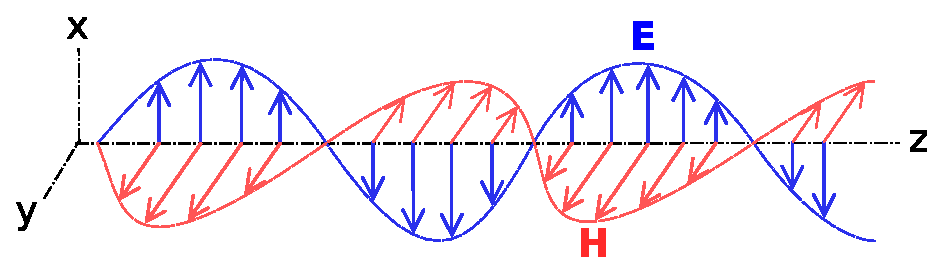
\includegraphics[width=\columnwidth]{modules/m0039_Onde_electromagnetique.eps}
% https://en.wikipedia.org/wiki/File:Onde_electromagnetique.svg
}}{Plotted on a three dimensional xyz coordinate system sits two sinusoidal waves perpendicular to one another. In the y-z plane sits the sinusoidal magnetic field wave. In the x-z plane sits the sinusoidal electric field wave. Each wave has vectors pointing from the axis to the wave.}
\end{center} 
\centerline{\scriptsize 
\copyright~\hyperref[m0039_Onde_electromagnetique_Credit]{E.\ Boutet} (Modified) 
\href{https://creativecommons.org/licenses/by-sa/3.0/}{CC BY~SA 3.0} 
} 
\caption{
\label{m0039_fPWR}
Relationship between the electric field direction, magnetic field direction, and direction of propagation (here, $+\hat{\bf z}$).
}
\end{figure}

If we observe this wave at some fixed point (i.e., hold $z$ constant), we find that the electric and magnetic fields are also periodic in time; specifically, they have the same value each time $t$ increases by $2\pi/\omega$.  We may characterize the speed at which the wave travels by comparing 
the distance required to experience $2\pi$ of phase rotation at a fixed time, which is $1/\beta$; to
the time it takes to experience $2\pi$ of phase rotation at a fixed location, which is $1/\omega$.  This is known as the {\it phase velocity}\footnote{We acknowledge that this is a misnomer, since velocity is properly defined as speed in a \emph{specified} direction, and $v_p$ by itself does not specify direction. In fact, the phase velocity in this case is properly said to be $+\hat{\bf z}v_p$.  Nevertheless, we adopt the prevailing terminology.} $v_p$:
\index{phase velocity}
%
\begin{equation}
v_p \triangleq \frac{1/\beta}{1/\omega} = \frac{\omega}{\beta} 
\end{equation}
%
Note that $v_p$ has the units expected from its definition, namely (rad/s)/(rad/m) $=$ m/s. If we make the substitution $\beta=\omega\sqrt{\mu\epsilon}$, we find
%
\begin{equation}
v_p = \frac{\omega}{\omega\sqrt{\mu\epsilon}} = \frac{1}{\sqrt{\mu\epsilon}}
\end{equation}
%
Note that $v_p$, like the wave impedance $\eta$, depends only on material properties.  
For example, the phase velocity of an electromagnetic wave in free space, given the special symbol $c$, is
%
\begin{equation}
c \triangleq \left. v_p \right|_{\mu=\mu_0, \epsilon=\epsilon_0} = \frac{1}{\sqrt{\mu_0\epsilon_0 }} \cong 3.00 \times 10^8~\mbox{m/s}
\end{equation}
%
This constant is commonly referred to as the \emph{speed of light}, 
\index{speed of light}
but in fact it is the phase velocity of an electromagnetic field at \emph{any} frequency (not just optical frequencies) in free space.  
Since the permittivity $\epsilon$ and permeability $\mu$ of any material is greater than that of a vacuum, $v_p$ in any material is less than the phase velocity in free space.
Summarizing:
%
%ORB HIGHLIGHT
\begin{mdframed}[backgroundcolor=yellow!20,nobreak=true] 
Phase velocity is the speed at which any point of constant phase appears to travel along the direction of propagation.
\end{mdframed}
%
%ORB HIGHLIGHT
\begin{mdframed}[backgroundcolor=yellow!20,nobreak=true] 
Phase velocity is maximum ($=c$) in free space, and slower by a factor of $1/\sqrt{\mu_r\epsilon_r}$ in any other lossless medium. 
\end{mdframed}

Finally, we note the following relationship between frequency $f$, wavelength, and phase velocity:
%
\begin{equation}
\lambda = \frac{2\pi}{\beta} 
= \frac{2\pi}{\omega / v_p}
= \frac{2\pi}{2\pi f / v_p}
= \frac{v_p}{f}
\end{equation}
%
Thus, given any two of the parameters $f$, $\lambda$, and $v_p$, we may solve for the remaining quantity.  
Also note that as a consequence of the inverse-proportional relationship between $\lambda$ and $v_p$, we find:
%
%ORB HIGHLIGHT
\begin{mdframed}[backgroundcolor=yellow!20,nobreak=true] 
At a given frequency, the wavelength in any material is shorter than the wavelength in free space.
\end{mdframed}

%%%%%%%%%%%%%%%%%%%%%%%%%%%%%%%%%%%%%%%%%%%%%%%
%ORB EXAMPLE
~\\ \begin{example} 
\begin{mdframed}[backgroundcolor=brown!20,linecolor=brown!20]\raggedright
Wave propagation in a lossless dielectric.
\index{dielectric (material)}
\\~\\
Polyethylene is a low-loss dielectric having $\epsilon_r \cong 2.3$.
What is the phase velocity in polyethylene?
What is wavelength in polyethylene?
The frequency of interest is 1~GHz.


{\bf Solution.}
Low-loss dielectrics exhibit $\mu_r \cong 1$ and $\sigma\approx 0$.
Therefore the phase velocity is
%
\begin{equation}
v_p = \frac{1}{\sqrt{\mu_0\epsilon_r\epsilon_0 }} = \frac{c}{\sqrt{\epsilon_r}} \cong 1.98 \times 10^8~\mbox{m/s}
\end{equation}
%
i.e., very nearly two-thirds of the speed of light in free space.
The wavelength at 1~GHz is
%
\begin{equation}
\lambda = \frac{v_p}{f} \cong 19.8~\mbox{cm}
\end{equation}
%
Again, about two-thirds of a wavelength at the same frequency in free space.

\end{mdframed}
% note figures will need to go between "\end{mdframed}" and "\end{example}"
\end{example}
%%%%%%%%%%%%%%%%%%%%%%%%%%%%%%%%%%%%%%%%%%%%%%%


Returning to polarization and magnitude, it is useful to note that Equation~\ref{m0039_eH2} could be written in terms of {\bf E} as follows:
%
\begin{equation}
{\bf H} = \frac{1}{\eta} \hat{\bf z} \times {\bf E} 
\end{equation}
%
i.e., ${\bf H}$ is perpendicular to both the direction of propagation (here, $+\hat{\bf z}$) and ${\bf E}$, with magnitude that is different from ${\bf E}$ by the wave impedance $\eta$.
%
This simple expression is very useful for quickly determining ${\bf H}$ given ${\bf E}$ when the direction of propagation is known.  
In fact, it is so useful that it commonly explicitly generalized as follows:
%
\begin{equation}
\boxed{
{\bf H} = \frac{1}{\eta} \hat{\bf k} \times {\bf E} 
}
\label{m0039_ePWRH}
\end{equation}
%
where $\hat{\bf k}$ (here, $+\hat{\bf z}$) is the direction of propagation.
Similarly, given ${\bf H}$, $\hat{\bf k}$, and $\eta$, we may find ${\bf E}$ using
%
\begin{equation}
\boxed{
{\bf E} = -\eta \hat{\bf k} \times {\bf H} 
}
\label{m0039_ePWRE}
\end{equation}
%
These spatial relationships can be readily verified using Figure~\ref{m0039_fPWR}.
%
%ORB HIGHLIGHT
\begin{mdframed}[backgroundcolor=yellow!20,nobreak=true] 
Equations~\ref{m0039_ePWRH} and \ref{m0039_ePWRE} are known as the \emph{plane wave relationships}.
\index{plane wave relationships}
\end{mdframed}
%
The plane wave relationships apply equally well to the phasor representations of ${\bf E}$ and ${\bf H}$; i.e.,
\begin{flalign}
\widetilde{\bf E} &= -\eta \hat{\bf k} \times \widetilde{\bf H} \\
\widetilde{\bf H} &= \frac{1}{\eta} \hat{\bf k} \times \widetilde{\bf E} 
\end{flalign}
%
These equations can be readily verified by applying the definition of the associated phasors (e.g., Equation~\ref{m0039_eEP}).
It also turns out that these relationships apply at each point in space, even if the waves are not planar, uniform, or in lossless media.

%%%%%%%%%%%%%%%%%%%%%%%%%%%%%%%%%%%%%%%%%%%%%%%
%ORB EXAMPLE
~\\ \begin{example} 
\begin{mdframed}[backgroundcolor=brown!20,linecolor=brown!20]\raggedright
Analysis of a radially-directed plane wave.
\\~\\
Consider the scenario illustrated in Figure~\ref{m0039_fEx1}.
Here a uniform plane wave having frequency $f=3$~GHz is propagating along a path of constant $\phi$, where is $\phi$ is known but not specified.  
The phase of the electric field is $\pi/2$~radians at $\rho=0$ (the origin) and $t=0$.
The material is an effectively unbounded region of free space.  
The electric field is oriented in the $+\hat{\bf z}$ direction and has peak magnitude of 1~mV/m.  
Find 
(a) the electric field intensity in phasor representation, 
(b) the magnetic field intensity in phasor representation, and 
(c) the actual, physical electric field along the radial path. 

{\bf Solution}: 
First, realize that this ``radially-directed'' plane wave is in fact a plane wave, and not a cylindrical wave.
It may well we be that if we ``zoom out'' far enough, we are able to perceive a cylindrical wave (for more on this idea, see Section~\ref{m0142_Types_of_Waves}), or it might simply be that wave is \emph{exactly} planar, and cylindrical coordinates just happen to be a convenient coordinate system for this application.
In either case, the direction of propagation $\hat{\bf k}=+\hat{\bf \rho}$ and the solution to this example will be the same.
 
Here's the phasor representation for the electric field intensity of a uniform plane wave in a lossless medium, analogous to Equation~\ref{m0039_eE}:
%
\begin{equation}
\widetilde{\bf E} = +\hat{\bf z}E_0 e^{-j\beta \rho} 
\end{equation}
%
From the problem statement, $\left|E_0\right| = 1$~mV/m.
Also from the problem statement, the phase of $E_0$ is $\pi/2$ radians; in fact, we could just write $E_0 = +j\left|E_0\right|$.
Thus, the answer to (a) is 
%
\begin{equation}
\widetilde{\bf E} = +\hat{\bf z}j\left|E_0\right| e^{-j\beta\rho}
\end{equation}
%
where the propagation constant $\beta = \omega\sqrt{\mu\epsilon} = 2\pi f \sqrt{\mu_0 \epsilon_0} \cong 62.9$~rad/m.  

The answer to (b) is easiest to obtain from the plane wave relationship:
%
\begin{flalign}
\widetilde{\bf H} &= \frac{1}{\eta} \hat{\bf k} \times {\bf E} \nonumber \\
                  &= \frac{1}{\eta} \hat{\bf \rho} \times \left( +\hat{\bf z}j\left|E_0\right| e^{-j\beta\rho} \right) \nonumber \\
                  &=-\hat{\bf \phi} \frac{j\left|E_0\right|}{\eta}  e^{-j\beta\rho} 
\end{flalign}
%
where $\eta$ here is $\sqrt{\mu_0/\epsilon_0} \cong 377~\Omega$. Thus, the answer to part (b) is
%
\begin{equation}
\widetilde{\bf H} = -\hat{\bf \phi}jH_0 e^{-j\beta\rho}
\end{equation}
%
where $H_0 \cong 2.65~\mu$A/m.
At this point you should check vector directions: $\widetilde{\bf E} \times \widetilde{\bf H}$ should point in the direction of propagation $+\hat{\bf \rho}$.
Here we find $\hat{\bf z} \times \left(-\hat{\bf \phi}\right) = +\hat{\bf \rho}$, as expected.

The answer to (c) is obtained by applying the defining relationship for phasors to the answer to part (a):
%
\begin{flalign}
{\bf E} &= \mbox{Re} \left\{ \widetilde{\bf E} e^{j\omega t} \right\}  \nonumber \\
        &= \mbox{Re} \left\{ \left(+\hat{\bf z}j\left|E_0\right| e^{-j\beta\rho}\right) e^{j\omega t} \right\}  \nonumber \\
        &= +\hat{\bf z} \left|E_0\right| \mbox{Re} \left\{ e^{j\pi/2} e^{-j\beta\rho} e^{j\omega t} \right\}  \nonumber \\
        &= +\hat{\bf z} \left| E_0 \right| \cos\left(\omega t - \beta\rho + \frac{\pi}{2} \right)
\end{flalign}
\end{mdframed}
%
\begin{figure}
\begin{center}
\pdftooltip{{  % note double braces
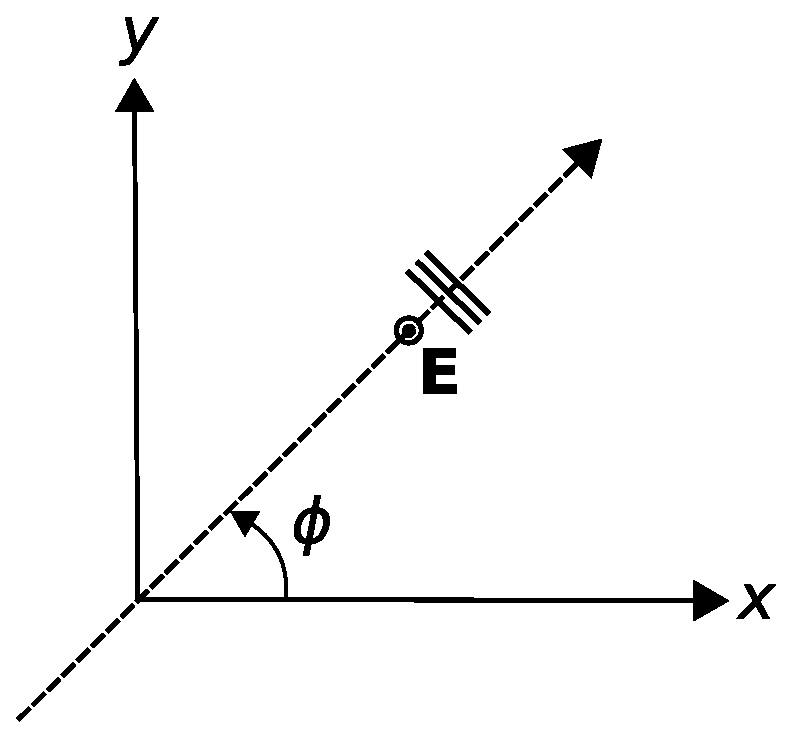
\includegraphics[width=2in]{modules/m0039_fEx1.eps}
% ***WikipediaCommonsURL
}}{An x-y plot with a dashed vector extending through the origin at an angle phi. On the vector at an arbitrary point is a circle, labeled E. Beside E on the vector are three straight parallel lines. }
\end{center} 
%\centerline{\scriptsize 
%\copyright~\hyperref[***_Credit]{author} 
%\href{https://creativecommons.org/licenses/by-sa/4.0/}{CC BY-SA 4.0} 
%} 
\caption{
\label{m0039_fEx1}
A radially-directed plane wave.
}
\end{figure}
\end{example}
%%%%%%%%%%%%%%%%%%%%%%%%%%%%%%%%%%%%%%%%%%%%%%%


{\bf Additional Reading:}
\begin{itemize}
\item ``\href{https://en.wikipedia.org/wiki/Electromagnetic_radiation}{Electromagnetic radiation}'' on Wikipedia.
\end{itemize}

\index{waves!plane|)}
